\chapter{Introduction}
\section{Motivation}
Since the introduction of Bitcoin, a peer-to-peer payment network and cryptocurrency, there have been countless new cryptocurrencies that are used and traded. Along with this, their high volatility has piqued a lot of retail investor's interest with some investors gaining a high return of interest and others losing a lot of money~\cite{losing_money_on_crypto_2021}. In addition to this, larger investment institutions have also sought to gain profits from this new type of tradable asset~\cite{gondek_what_nodate}. This has lead to more sophisticated forms of cryptocurrency trading.
\\[5mm]
However, trading cryptocurrencies was initially very difficult for people without technical know-how, and the first recorded transaction was on $12^{th}$ October 2009 via a paypal transaction~\cite{noauthor_history_nodate}. Since then, other cryptocurrency exchanges have emerged, many of which are centralized, which provide a more traditional trading terminal and support for investors with little technical know-how, and others are decentralised, which operate on blockchain networks and allow users to directly with each other using smart contracts. Centralized exchanges are predominant due to their easy-to use and familiar interface for traders. We can see in Figure \ref{fig:dex_to_cex} the proportion of trades on decentralised exchanges compares to the number of trades on centralized exchanges, we can also see that the volume traded in decentralised exchanges (DEXes) have been near 0\% until the summer of 2020 and has been increasing since. 

\begin{figure}[htb!]
    \centering
    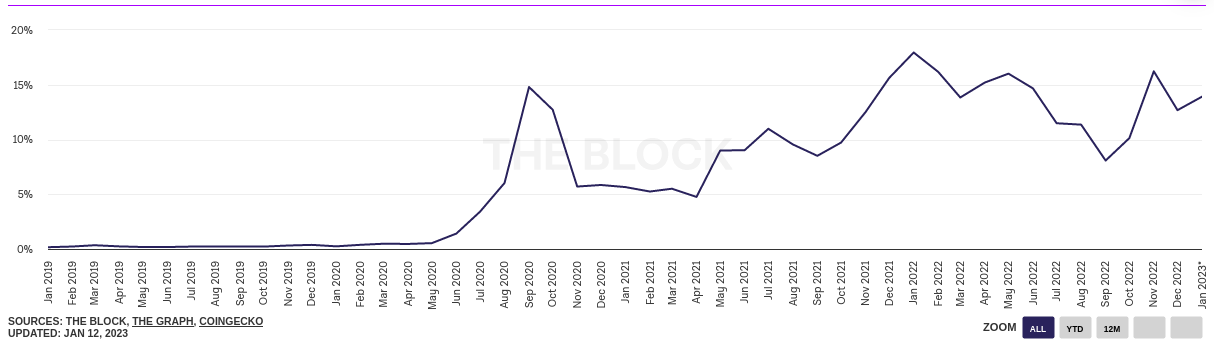
\includegraphics[width=\textwidth]{introduction/Images/dex_to_cex.png}
    \caption{{DEX} to {CEX} {Spot} {Trade} {Volume}~\cite{dex_to_cex}}
    \label{fig:dex_to_cex}
\end{figure}

This poses the question that about which trading strategies can exploit arbitrage opportunities on decentralised exchanges. There has been some research on this topic, mainly focussing on triangular and cyclic arbitrage on DEXes such as Uniswap and SushiSwap, however there has been no research into analysing the performance of statistical arbitrage methods on decentralised exchanges.

\section{Ethical Issues}

The ethics of cryptocurrencies are widely debated for reasons such as anonymity, leading it to be the choice of currency used by criminals and illegal institutions, volatility and lack of regulation. The high volatility makes cryptocurrencies and decentralised finance very risky for retail investors that don't have the technical or financial know-how making investing in cryptocurrencies.
\\[5mm]
Another aspect of cryptocurrencies that has raised ethical questions is the energy consumption and carbon dioxide emission from the mining of cryptocurrencies. Formal research about this has also been completed and found that `approximately 69 million metric tons of CO2 (Carbon dioxide) emission as a result of bitcoin mining'~\cite{egiyi2020cryptocurrency}. Thus, this is an ethical concern that I have thought about when designing the strategies so that the number of transactions that don't result in a profit, i.e. do not add value to the project, is limited.
\\[5mm]
In addition to the concerns above, although this project aims to find riskless profits, \textit{`free lunches'}, it is not, in any form, of financial advice, and those who use the research or software that used in the development and research process to attempt to get favourable results, are liable for the losses or gains. 



\section{Contributions - TODO}